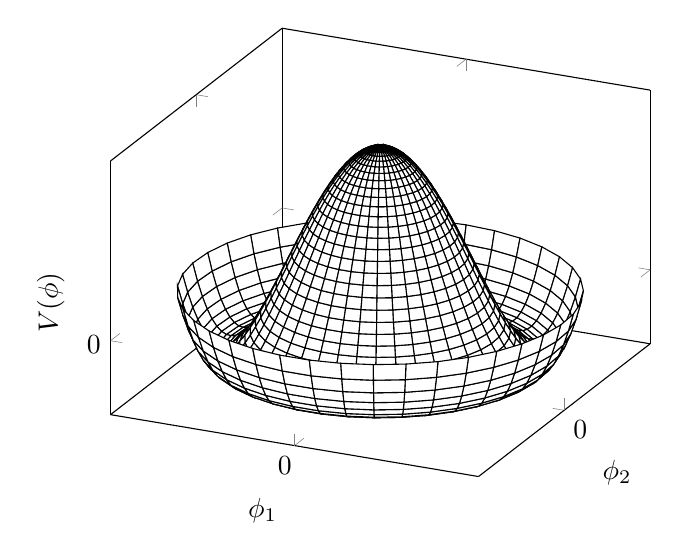
\begin{tikzpicture}

    \begin{axis}[
        xlabel = $\phi_1$,
        ylabel = $\phi_2$,
        zlabel = $V(\phi)$,
        xtick={0},
        ytick={0},
        ztick={0},
        samples=40,
        domain=0:360,
        y domain=0:1.25,
    ]
    %\addplot3 [surf, shader=flat, draw=black, fill=white, z buffer=sort] ({sin(x)*y}, {cos(x)*y}, {(y^2-1)^2});
    \addplot3 [surf, shader=flat, draw=black, fill=white, z buffer=sort] ({sin(x)*y}, {cos(x)*y}, {(y^2-1)^2} - 0.25);

    \end{axis}

\end{tikzpicture}